\chapter{Beyond the Buzzwords: What AI Actually Means for Your Business}

\epigraph{The greatest enemy of knowledge is not ignorance, it is the illusion of knowledge.}{Stephen Hawking}

\section{The Many Meanings of ``AI''}

Every quarter, someone walks into a board meeting with a slide deck featuring ``AI-powered'' solutions. The term has been stretched to cover everything from spam filters to autonomous vehicles. This creates confusion---and confusion is expensive. When a vendor says ``AI-powered,'' they might mean:

\begin{itemize}
    \item \textbf{Rule-based systems:} Software following explicit if-then logic. Traditional, not really AI in the modern sense.
    \item \textbf{Machine learning:} Systems that learn patterns from data to make predictions.
    \item \textbf{Deep learning:} Neural networks that can handle complex patterns like images and language.
    \item \textbf{Generative AI:} Systems that create new content---text, images, code, audio.
\end{itemize}

For this book, we focus primarily on generative AI and its practical business applications, because that is where the immediate opportunities lie for most executives. When you hear about ChatGPT, Claude, Copilot, or similar tools at industry conferences, you are hearing about generative AI.

\begin{figure}[htbp]
\centering
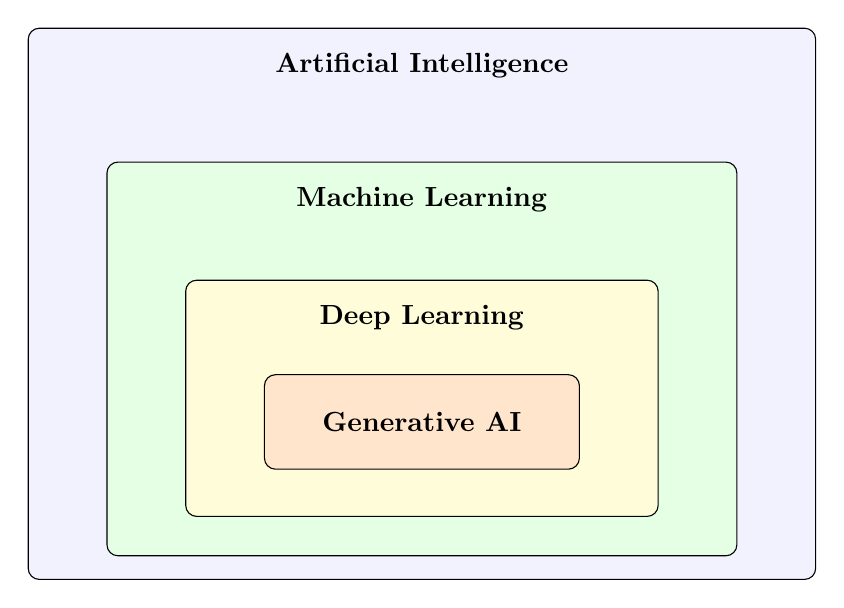
\begin{tikzpicture}
    % Outermost box - AI
    \node[draw, rounded corners, minimum width=10cm, minimum height=7cm, fill=blue!5] (ai) {};
    \node[anchor=north] at ([yshift=-0.2cm]ai.north) {\textbf{Artificial Intelligence}};

    % Machine Learning box
    \node[draw, rounded corners, minimum width=8cm, minimum height=5cm, fill=green!10] at ([yshift=-0.7cm]ai.center) (ml) {};
    \node[anchor=north] at ([yshift=-0.2cm]ml.north) {\textbf{Machine Learning}};

    % Deep Learning box
    \node[draw, rounded corners, minimum width=6cm, minimum height=3cm, fill=yellow!15] at ([yshift=-0.5cm]ml.center) (dl) {};
    \node[anchor=north] at ([yshift=-0.2cm]dl.north) {\textbf{Deep Learning}};

    % Generative AI box
    \node[draw, rounded corners, minimum width=4cm, minimum height=1.2cm, fill=orange!20] at ([yshift=-0.3cm]dl.center) (gen) {};
    \node at (gen.center) {\textbf{Generative AI}};
\end{tikzpicture}
\caption{The relationship between AI, machine learning, deep learning, and generative AI}
\label{fig:ai-hierarchy}
\end{figure}

\section{From Rules to Predictions: A Fundamental Business Shift}

Traditional business software follows rules: ``If customer spent over \$1000, offer 10\% discount.'' Someone on your team defined that rule. The software executes it.

AI systems work differently. You show them thousands of examples: customers who responded well to discounts, customers who did not. The system identifies patterns you never explicitly defined. Maybe it discovers that customers who browse on mobile devices on Sunday evenings respond better to free shipping than percentage discounts---an insight no analyst thought to look for.

This shift from ``rules we write'' to ``patterns the system discovers'' is the core mental model to understand. It changes how you think about business process optimization, customer insights, and competitive intelligence.

\begin{table}[htbp]
\centering
\begin{tabularx}{\textwidth}{lXX}
\toprule
\textbf{Aspect} & \textbf{Traditional Software} & \textbf{AI/ML Systems} \\
\midrule
Logic & Rules written by humans & Patterns learned from data \\
Changes & Requires code updates & Can adapt with new data \\
Predictions & Deterministic, same input = same output & Probabilistic, may vary \\
Edge cases & Must be explicitly handled & May generalize (or fail) \\
Explainability & Clear, traceable logic & Often opaque \\
\bottomrule
\end{tabularx}
\caption{Comparing traditional software and AI systems}
\end{table}

\section{What Generative AI Really Does}

Generative AI predicts what should come next.

When you ask ChatGPT a question, it is predicting: ``Given this question, what response would most likely follow based on billions of examples I learned from?'' It is not ``thinking'' or ``understanding'' in the human sense. It is sophisticated pattern matching at unprecedented scale.

This explains both its strengths and failures:

\begin{itemize}
    \item \textbf{It sounds fluent} because it learned from fluent text
    \item \textbf{It can be confidently wrong} because ``sounding right'' and ``being right'' are different things
    \item \textbf{It struggles with novel reasoning} because it relies on patterns, not genuine understanding
\end{itemize}

\begin{keyinsight}
Think of generative AI as the world's most sophisticated autocomplete. It is remarkably good at predicting what text should come next based on patterns. But prediction is not understanding, and fluency is not accuracy. This distinction drives every decision about when to use AI and when to rely on human judgment.
\end{keyinsight}

\section{Where AI Is Already Around You}

Before you ``adopt AI,'' recognize you are already using it:

\begin{table}[htbp]
\centering
\begin{tabular}{ll}
\toprule
\textbf{Service} & \textbf{AI Application} \\
\midrule
Email spam filtering & Classification ML \\
Netflix recommendations & Recommendation systems \\
Google search results & Ranking algorithms + LLMs \\
Phone face unlock & Computer vision \\
Credit card fraud alerts & Anomaly detection \\
Autocorrect/autocomplete & Language models \\
\bottomrule
\end{tabular}
\caption{AI you already use daily}
\end{table}

The question is not whether to use AI---it is whether to use it more deliberately and strategically.

\section{Why This Time Is Different: The Business Case}

Previous AI hype cycles (2015, 2018) promised transformations that did not materialize for most businesses. Executives who ignored those waves often looked wise. This time is different, and here is why:

\textbf{Accessibility changed.} You no longer need a data science team to use AI. ChatGPT, Claude, and Copilot work through natural language. If you can describe what you want, you can use these tools. Your marketing director can use AI today---no IT ticket required.

\textbf{Capabilities crossed a threshold.} Pre-2022 language models were interesting but not business-ready. Current models can draft contracts, analyze financial reports, prepare board presentations, and summarize complex documents at a level that is genuinely useful.

\textbf{Cost dropped dramatically.} What cost thousands in computing three years ago now costs pennies per task. The unit economics changed fundamentally.

\textbf{The competitive pressure is real.} Your competitors are using these tools. The productivity gap between AI-assisted and non-AI-assisted work is widening. Early adopters are pulling ahead in operational efficiency.

\begin{realexample}[The Productivity Gap]
A professional services firm tracked two teams doing similar client analysis work. The team using AI tools consistently delivered reports 40\% faster with comparable quality. After six months, the difference in client capacity was significant. The AI-assisted team could handle more engagements, leading to higher revenue per consultant and better client satisfaction scores. The firm is now rolling out AI tools company-wide.
\end{realexample}

\section{What This Book Will and Will Not Cover}

\textbf{Will cover:}
\begin{itemize}
    \item Using existing AI tools effectively (ChatGPT, Claude, Copilot, specialized tools)
    \item Evaluating when AI is appropriate for a task
    \item Managing AI risks (accuracy, privacy, bias)
    \item Implementing concrete AI projects with measurable results
    \item Building organizational capability over time
\end{itemize}

\textbf{Will not cover:}
\begin{itemize}
    \item Building custom AI models from scratch
    \item Technical ML/DL theory
    \item AI for highly specialized domains (medical diagnosis, autonomous vehicles)
    \item Speculative future capabilities
\end{itemize}

\section{Summary}

AI is not magic. It is a set of prediction and pattern-recognition tools that turn data into useful business outputs. Generative AI creates new content---text, analysis, presentations---from patterns it has learned.

The shift from rule-based software to pattern-based AI represents a fundamental change in how businesses can operate. But leveraging this shift requires knowing both what AI does well and where it fails.

You are already using AI every day, whether you realize it or not. The strategic question now is whether to use it more deliberately, more systematically, and more competitively. That starts with understanding how AI systems actually ``think''---which is the subject of our next chapter.

\begin{exercise}
List five AI-powered services you use in a typical week. For each, identify what the AI is actually doing (classification, prediction, generation, recommendation).
\end{exercise}

\begin{exercise}
Find three ``AI-powered'' products in your industry. Research what kind of AI they actually use. Are they using generative AI, machine learning for predictions, or something else?
\end{exercise}
